\begin{frame}
	\frametitle{Introduction}
	
	Goal: Calculation of gravitational force on a system of collisionless particles
	
	Possible methods:
	
	\begin{itemize}
		\item Direct calculation
		\item Iterative methods on a mesh
		\item Fourier methods on a mesh
		\item Tree methods (hierarchical multipole methods)
	\end{itemize}

	In this project, I implemented a direct calculation and a tree method.
\end{frame}







\begin{frame}
	\frametitle{Dataset}
	The dataset for which to compute the forces is a set of $\sim 50'000$ particles aranged according to the spherically symmetric ``Hernquist model'' :
	\begin{align*}
		\rho(r) &= \frac{M}{2\pi}\frac{a}{r}\frac{1}{(r+a)^3}\\
		M(r) &= M \frac{r^2}{(r+a)^2} \quad\quad \Rightarrow M(a) = \frac{M}{4}\\
		\phi(r) &= - \frac{GM}{r+a}
	\end{align*}
\end{frame}




\begin{frame}
	\frametitle{Choice of Units}
	
	Use dimensionless units, with $G \equiv 1$
	
	$\Rightarrow$ Reduce number of multiplications necessary
	
	$\Rightarrow$ Reduce effect of finite floating point precision by moving problem to a better suited order of magnitude
	
	Define a scale for every physical quantity:
	\begin{align*}
		a_{phys} \equiv A_0 a_{code}
	\end{align*}
	
	Setting $G = 1$ restricts the scale for either time, mass or distance. I chose
	\begin{align*}
		M_0 &= M_{tot}	\quad\quad &\text{ such that } \quad M_{tot, code} = 1\\
		R_0 &= R_{max}	\quad\quad &\text{ such that } \quad R_{max, code} = 1\\
		\Rightarrow \quad T_0 &= \sqrt{ \frac{R_0^3}{G M_0}} &
	\end{align*}
	
\end{frame}





\begin{frame}
	\frametitle{Dataset}
	\centering
	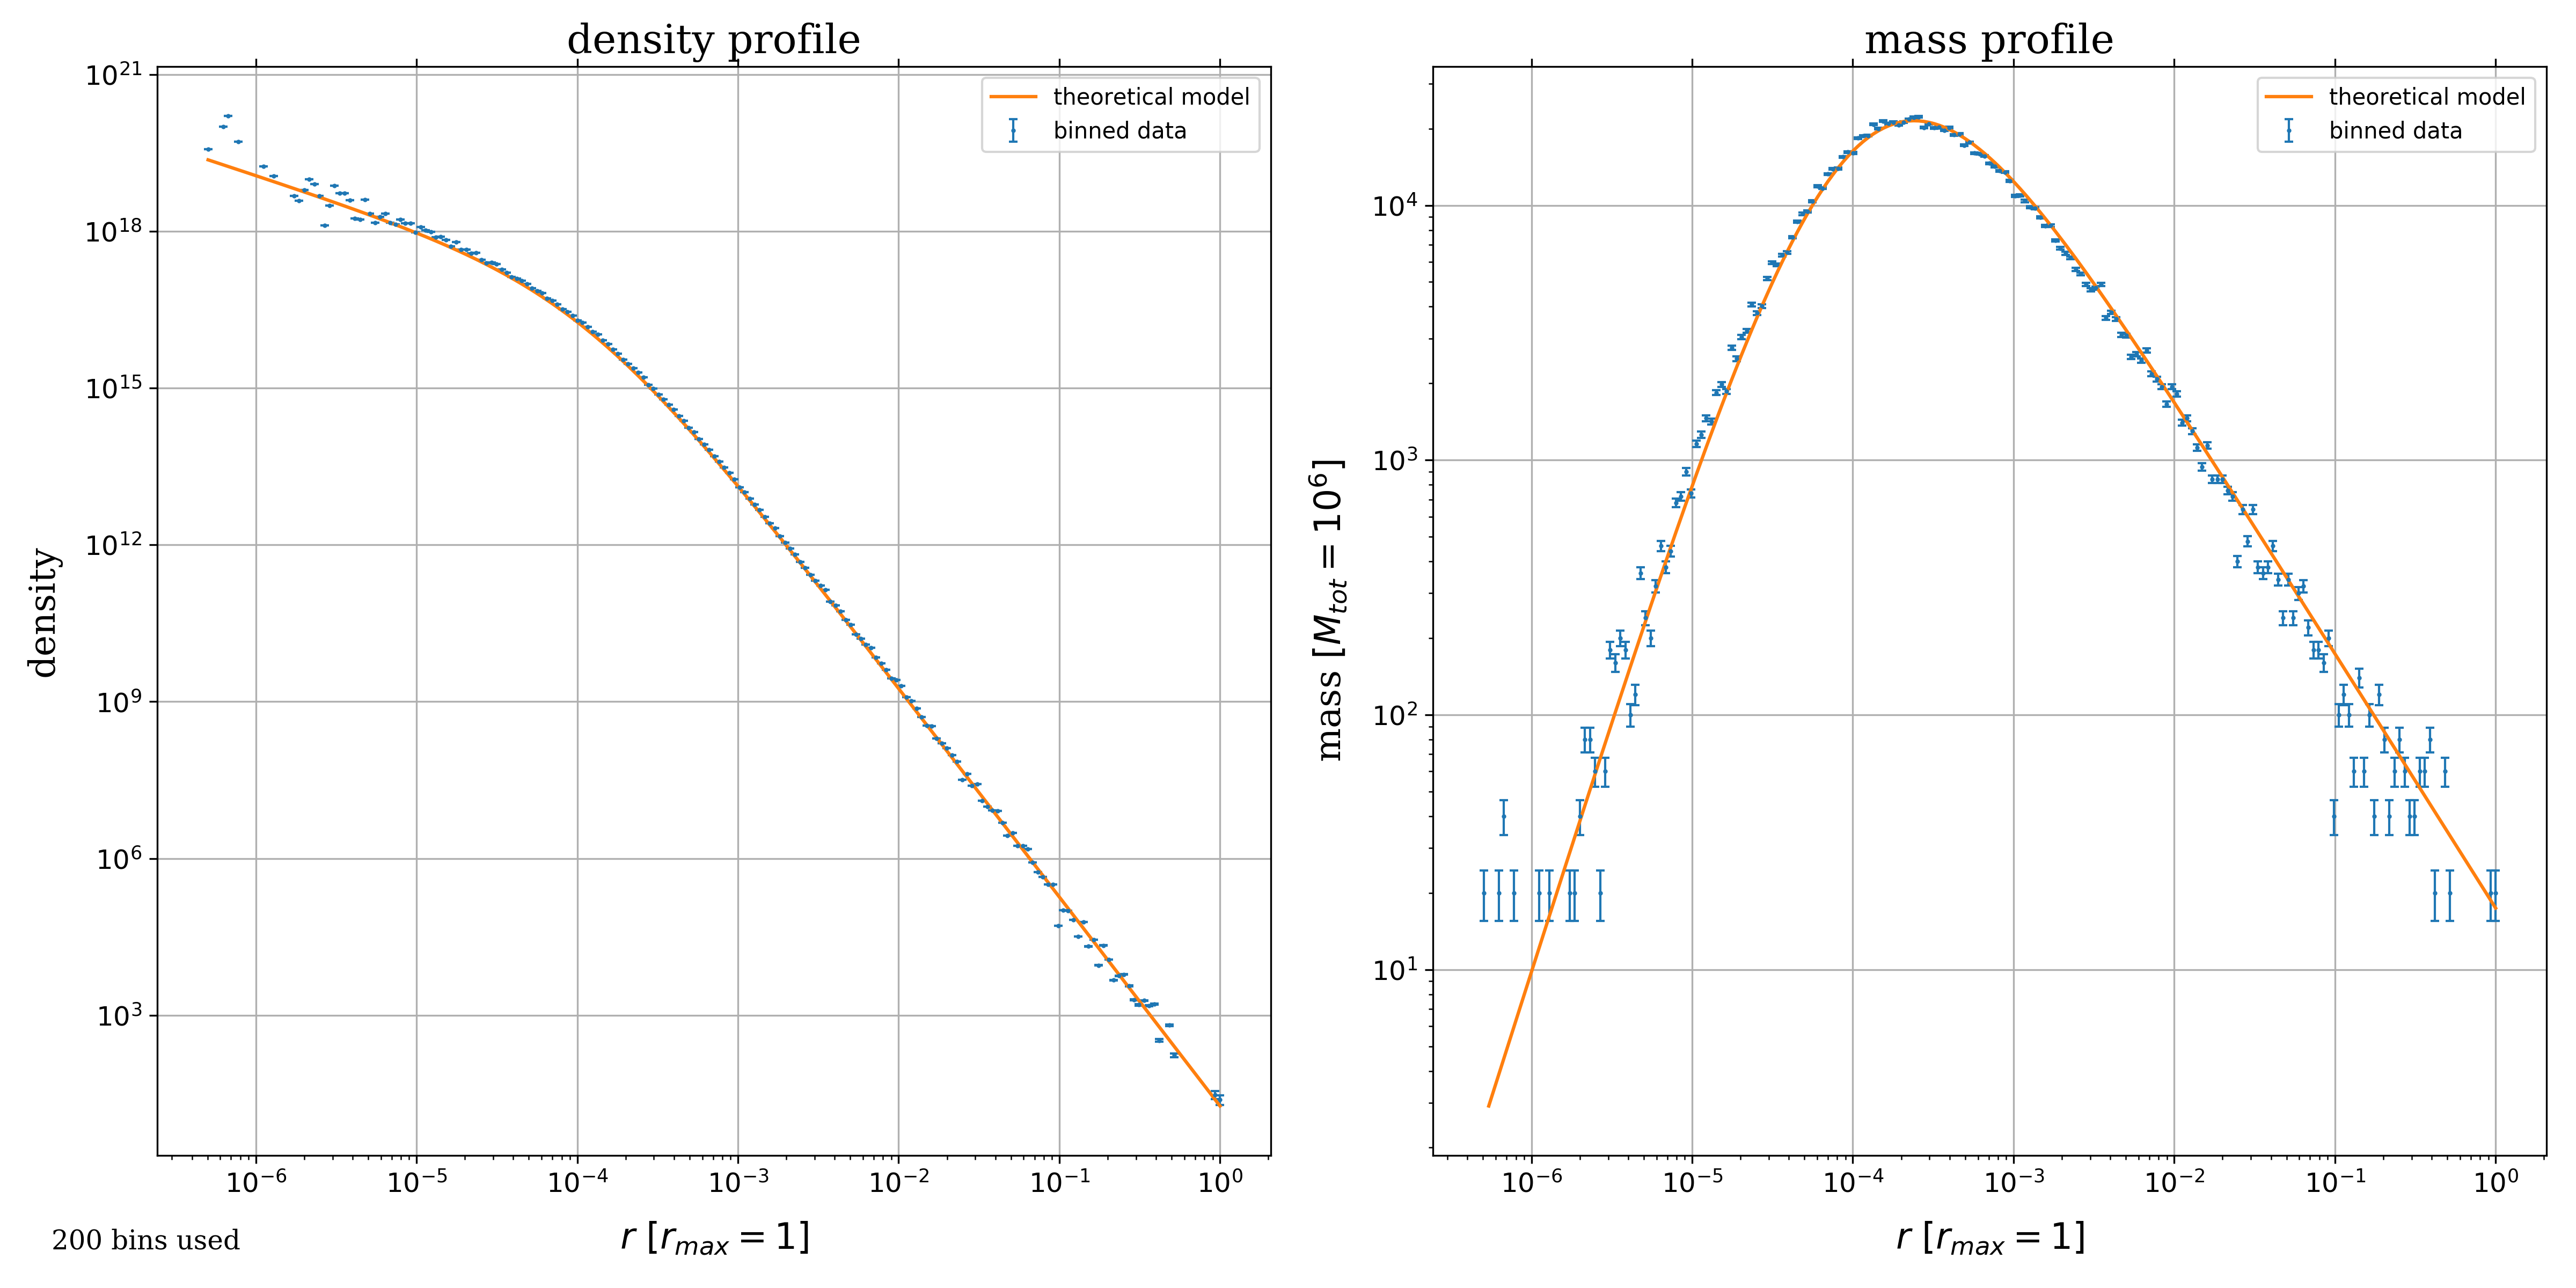
\includegraphics[width=\linewidth]{../results/density_plot/step0_density_plot.png}
	
	\alert{Only in this plot:} $M_{tot} \equiv 10^6$ so that the errorbars don't dominate the plot.
\end{frame}



